\documentclass{book}

\usepackage{graphicx,epsfig}
\usepackage{hyperref}
\usepackage{amsmath,amssymb}
\usepackage[toc,page]{appendix}
\usepackage{tikz}
\usetikzlibrary{shapes.geometric, arrows.meta, positioning, fit, backgrounds}
\usepackage{booktabs}
\usepackage{array}
\usepackage{multirow}
\usepackage{enumitem}
\usepackage{geometry}

\geometry{
  textheight=9in,
  textwidth=6.5in,
  headheight=0in,
  headsep=0in,
  topmargin=0in,
  oddsidemargin=0in,
  evensidemargin=0in
}

\setlength{\parindent}{.3in}
\renewcommand{\baselinestretch}{1}
\pagestyle{plain}

% Compact list spacing
\setlist[itemize]{noitemsep, topsep=2pt, parsep=0pt, partopsep=0pt}
\setlist[enumerate]{noitemsep, topsep=2pt, parsep=0pt, partopsep=0pt}

% TikZ styles for flowcharts
\tikzstyle{block} = [rectangle, rounded corners, minimum width=2.2cm, minimum height=0.55cm,
    text centered, draw=black, fill=blue!10, font=\small]
\tikzstyle{arrow} = [thick,->,>=stealth]
\tikzstyle{decision} = [diamond, aspect=2, minimum width=2cm, minimum height=0.5cm,
    text centered, draw=black, fill=yellow!20, font=\scriptsize]

\begin{document}
\bibliographystyle{plain}

\large

%% ============================================================
%% TITLE PAGE
%% ============================================================
\thispagestyle{empty}
\centerline{\bf A REPORT}
\vspace*{0.3cm}
\centerline{\bf ON}
\vspace*{0.3cm}
\centerline{\bf SWECHA PS-I PROJECT PORTFOLIO: HIGHONCODE TEAM PORTFOLIO,}
\centerline{\bf MEOWBOT AI X, ADHIKARSETU AND SMART STOCK DASHBOARD}
\vspace*{2cm}

\centerline{BY}
\vspace*{1cm}

\begin{center}
  \begin{tabular}{lll}
    Name of the student & \hspace*{1.5cm} ID No. & \hspace*{1.5cm} Discipline \\
    Soumyajit Rout & \hspace*{1.5cm} 2024A7PS0002P & \hspace*{1.5cm} B.E. Computer Science \\
  \end{tabular}
\end{center}

\vspace*{2cm}
\begin{center}
  {\bf Prepared in partial fulfillment of the \\
  Practice School - I}
\end{center}

\vspace*{0.5cm}
\centerline{AT}
\vspace*{1cm}
\centerline{\bf Swecha Telangana, Hyderabad}
\vspace{0.2cm}
\centerline{\bf A Practice School - I}
\vspace{0.2cm}
\centerline{\bf Station of}
\vspace{0.5cm}
\begin{figure}[ht]
\epsfxsize=1.0in
\centerline{\epsffile{logo.eps}}
\end{figure}

\centerline{\bf BIRLA INSTITUTE OF TECHNOLOGY \& SCIENCE, PILANI}
\vspace*{0.5cm}
\centerline{\bf June, 2026}
\newpage

%% ============================================================
%% PS DIVISION SUMMARY SHEET
%% ============================================================
\thispagestyle{empty}
\centerline{\bf BIRLA INSTITUTE OF TECHNOLOGY \& SCIENCE, PILANI}
\vspace*{0.2cm}
\centerline{\bf Practice School Division}
\vspace*{0.3cm}
{\bf
\begin{tabular}{p{5.5cm}p{7.5cm}}
  & \\
  Station & Swecha Telangana \\
  & \\
  Duration & May -- June 2026 \quad Date of start: May 2026 \\
  & \\
  Date of submission & 20 June 2026 \\
  & \\
  Title of the project: & Swecha PS-I Project Portfolio: HighOnCode Team Portfolio,
    MeowBot AI X, AdhikarSetu and Smart Stock Dashboard \\
  & \\
  ID No., Name and Discipline: & 2024A7PS0002P, Soumyajit Rout, B.E. Computer Science \\
  & \\
  Name and Designation of the expert: & Swecha Telangana Mentor \\
  & \\
  Name of the PS faculty member: & Dr.\ Tanmay Chatterjee \\
  & \\
  Key words: & Artificial Intelligence, Retrieval Augmented Generation, Natural Language
    Processing, Machine Learning, Stock Prediction, FastAPI, React, Next.js, Streamlit,
    Financial Analytics, Government Scheme Recommendation, Data Visualization,
    Portfolio Website, Frontend Engineering, Deployment \\
  & \\
  Project area(s): & Artificial Intelligence, Machine Learning, NLP, Financial Analytics,
    Frontend Development, Backend Development, Full Stack Development,
    Retrieval-Augmented Generation, Government Technology, Data Visualization \\
  & \\
  Abstract: & This report presents work completed during Practice School-I at Swecha
    Telangana between May and June 2026. Four projects were completed, spanning frontend
    engineering, backend development, machine learning, natural language processing, and
    deployment. Project 1, HighOnCode Team Portfolio, is an immersive SSR portfolio
    website built with React 19, TanStack Start, GSAP, and Framer Motion, deployed on
    Cloudflare Workers. Project 2, Document Intelligence Chatbot (MeowBot AI X), is a
    RAG-based assistant combining ChromaDB, Sentence Transformers, Groq Llama, and
    Streamlit with NLP analytics. Project 3, AdhikarSetu, is a hackathon platform for
    MSME scheme discovery where I developed the complete frontend, three backend APIs,
    and handled deployment. Project 4, Stock Intelligence Dashboard, is a
    production-grade ML-driven financial analytics platform built with FastAPI, React,
    scikit-learn, Supabase, and a multi-provider BYOK AI chat system. \\
  & \\
  Signature of the student & \hspace*{1cm} Signature of the PS faculty member \\
  & \\
  Date & \hspace*{1cm} Date \\
\end{tabular}}

\newpage

%% ============================================================
%% ACKNOWLEDGEMENTS
%% ============================================================
\centerline{\bf \Large Acknowledgements}
\vspace*{0.5cm}

\par\noindent I would like to express my sincere gratitude to the mentors and coordinators at Swecha Telangana for providing a stimulating environment for project-based learning and open-source development during Practice School-I.

\par\noindent I am grateful to Dr.\ Tanmay Chatterjee, PS Faculty-in-Charge, for his guidance and support throughout the duration of this practice school. I also thank the BITS Pilani Practice School Division for organizing this programme.

\par\noindent For Project 3, AdhikarSetu, I acknowledge my two teammates for their collaboration. In particular, I credit the scheme matching engine to a fellow team member, as clearly noted in the report.

\par\noindent Finally, I thank the open-source communities behind React, FastAPI, scikit-learn, ChromaDB, TanStack, and all other tools used across these projects.

\vfill
\par\noindent {\bf Signature of the student}

\tableofcontents
\listoffigures
\listoftables

%% ============================================================
%% CHAPTER 1: INTRODUCTION
%% ============================================================
\chapter{Introduction}

\par\noindent Practice School-I (PS-I) at Swecha Telangana, Hyderabad, provided an opportunity to apply classroom knowledge to real-world software engineering challenges. Over the course of May and June 2026, four projects were conceptualized, designed, developed, and deployed, spanning the domains of frontend engineering, retrieval-augmented generation, civic technology, and financial analytics.

\par\noindent This report is organized chronologically and presents each project in a self-contained section covering its objectives, architecture, methodology, results, and future scope. In addition, a dedicated section summarizes the technical learning and professional development gained through seminars, workshops, and self-directed study conducted during the PS-I period.

\section{Overview of Projects}

\par\noindent The four projects completed during PS-I are listed below.

\begin{enumerate}
  \item \textbf{HighOnCode Team Portfolio} (May 2026) --- An immersive, single-page SSR portfolio website for a three-member engineering collective, featuring a cinematic deep-ocean theme, GSAP and Framer Motion animations, and Cloudflare Workers deployment.
  \item \textbf{Document Intelligence Chatbot (MeowBot AI X)} (May 2026) --- A RAG-based document assistant combining semantic search, conversational question answering, and automated NLP analytics over uploaded PDF documents.
  \item \textbf{AdhikarSetu} (May--June 2026) --- A group hackathon project providing MSME owners with government scheme discovery, benefit estimation, and rejection explanation through a full-stack web platform.
  \item \textbf{Stock Intelligence Dashboard} (May--June 2026) --- A production-ready, ML-driven stock analysis and prediction platform integrating scikit-learn ensemble models, a multi-provider BYOK AI chat system, and multilingual support.
\end{enumerate}

%% ============================================================
%% CHAPTER 2: HIGHONCODE TEAM PORTFOLIO
%% ============================================================
\chapter{HighOnCode Team Portfolio}

\section{Project Overview and Objective}

\par\noindent \textbf{Project Title:} HighOnCode Team Portfolio\\
\textbf{Live URL:} \href{https://highoncode.vercel.app}{highoncode.vercel.app}

\par\noindent \textbf{Problem Statement:} Engineering teams often lack a cohesive, visually compelling online presence that simultaneously communicates technical depth, individual contributions, and collaborative philosophy. Standard portfolio templates fail to convey the personality and engineering culture of a team.

\par\noindent \textbf{Objective:} To design and deploy a production-grade, single-page SSR portfolio website for HighOnCode, a three-member BITS Pilani engineering collective, using modern React meta-frameworks and cinematic frontend animations. I was the sole developer of the project.

\section{System Architecture and Tech Stack}

\par\noindent The application was built as a single-page SSR application using TanStack Start as the meta-framework with React 19, providing file-based routing and full server-side rendering. Table~\ref{tab:hoc_stack} summarizes the technology stack.

\begin{table}[!h]
\begin{center}
\small
\begin{tabular}{|l|l|}
\hline
\textbf{Category} & \textbf{Technology} \\
\hline
Meta-framework & TanStack Start + TanStack Router \\
UI Library & React 19 \\
Language & TypeScript \\
Styling & Tailwind CSS v4 \\
Animation & GSAP, Framer Motion \\
Smooth Scroll & Lenis \\
Deployment & Cloudflare Workers (via Nitro adapter) \\
\hline
\end{tabular}
\caption{HighOnCode Portfolio -- Technology Stack}
\label{tab:hoc_stack}
\end{center}
\end{table}

\par\noindent Cloudflare Workers served as the serverless runtime for SSR, with the Nitro adapter bridging TanStack Start's build output to the Workers environment. No database or backend API was required.

\section{Methodology and Implementation}

\par\noindent Although AI-assisted tooling (Lovable, GitHub Copilot) was used during initial scaffolding, the entire application was subsequently redesigned, animated, debugged, and deployed by me. Every component, animation sequence, layout, and interaction was hand-crafted to match the desired aesthetic.

\par\noindent The website is organized into eight sections: (1) Hero with animated headline and magnetic CTA button; (2) Identity, presenting team philosophy; (3) Team, featuring interactive dossier cards with Overview, Skills, Projects, Achievements, and Contact tabs; (4) Skills, with a radar chart and proficiency bars; (5) Learning; (6) Workflow; (7) Fun Zone with statistics and team chemistry visualizations; and (8) Footer.

\par\noindent The visual design follows a cinematic deep-ocean aesthetic. The color palette uses dark blue, cyan, teal, and bioluminescent accents. Signature effects include floating bubble animations, animated fish and jellyfish SVGs, caustic lighting, sonar ring pulses, scan-line overlays, and wave dividers. A custom fish cursor with inertia and ambient audio support were also implemented.

\par\noindent Adaptive motion profiles were integrated to automatically reduce animation complexity for low-end devices, touch devices, and users with \texttt{prefers-reduced-motion} enabled, ensuring accessibility compliance.

\section{Results and Practical Applications}

\par\noindent The completed website successfully presents the team's technical portfolio in a visually distinctive format. The SSR architecture ensures fast initial load and good SEO characteristics. The project demonstrated proficiency in modern React meta-frameworks, advanced CSS animation, GSAP timeline orchestration, Framer Motion gesture physics, and serverless SSR deployment.

\par\noindent \textbf{Future Enhancements:} Integration of a CMS for content updates, Lighthouse performance benchmarking, and expansion of the dossier system to support dynamic project data fetched from GitHub APIs.

%% ============================================================
%% CHAPTER 3: DOCUMENT INTELLIGENCE CHATBOT
%% ============================================================
\chapter{Document Intelligence Chatbot}

\section{Project Overview and Objective}

\par\noindent \textbf{Project Title:} Document Intelligence Chatbot (MeowBot AI X)\\
\textbf{Repository:} \href{https://code.swecha.org/soumyajit_07/meowbot}{code.swecha.org/soumyajit\_07/meowbot}

\par\noindent \textbf{Problem Statement:} Large PDF documents such as research papers, technical reports, and manuals are difficult to navigate manually. Users spend considerable time extracting relevant insights without any intelligent assistance.

\par\noindent \textbf{Objective:} To build a RAG-based document intelligence assistant that allows users to upload PDFs, query them through natural language, and receive automatically generated analytics including keyword extraction, entity recognition, sentiment analysis, readability assessment, and semantic clustering.

\section{System Architecture and Tech Stack}

\begin{table}[!h]
\begin{center}
\small
\begin{tabular}{|l|l|}
\hline
\textbf{Component} & \textbf{Technology} \\
\hline
Embedding Model & SentenceTransformer all-MiniLM-L6-v2 (384-dim) \\
Vector Database & ChromaDB (local persistent, HNSW, cosine similarity) \\
Primary LLM & Groq llama-3.3-70b-versatile \\
Secondary LLMs & llama-3.1-8b-instant (Groq), llama3.2 (Ollama), OpenAI \\
Keyword Extraction & KeyBERT with Maximum Marginal Relevance \\
NLP & spaCy (NER), HuggingFace (sentiment), textstat (readability) \\
Visualization & Plotly \\
UI Framework & Streamlit \\
\hline
\end{tabular}
\caption{Document Intelligence Chatbot -- Technology Stack}
\label{tab:meow_stack}
\end{center}
\end{table}

\section{Methodology and RAG Workflow}

\par\noindent Figure~\ref{fig:rag_flow} illustrates the end-to-end RAG pipeline.

\begin{figure}[ht]
\centering
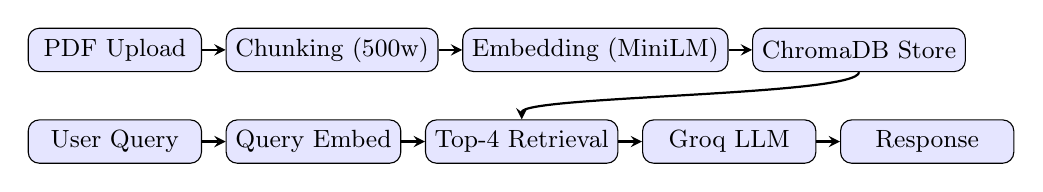
\begin{tikzpicture}[node distance=0.45cm and 0.3cm]
  \node (upload) [block] {PDF Upload};
  \node (chunk)  [block, right=of upload] {Chunking (500w)};
  \node (embed)  [block, right=of chunk] {Embedding (MiniLM)};
  \node (store)  [block, right=of embed] {ChromaDB Store};
  \node (query)  [block, below=0.6cm of upload] {User Query};
  \node (qembed) [block, right=of query] {Query Embed};
  \node (ret)    [block, right=of qembed] {Top-4 Retrieval};
  \node (llm)    [block, right=of ret] {Groq LLM};
  \node (resp)   [block, right=of llm] {Response};

  \draw[arrow] (upload) -- (chunk);
  \draw[arrow] (chunk)  -- (embed);
  \draw[arrow] (embed)  -- (store);
  \draw[arrow] (query)  -- (qembed);
  \draw[arrow] (qembed) -- (ret);
  \draw[arrow] (store.south) .. controls +(0,-0.3) and +(0,0.3) .. (ret.north);
  \draw[arrow] (ret)    -- (llm);
  \draw[arrow] (llm)    -- (resp);
\end{tikzpicture}
\caption{RAG Pipeline -- Document Intelligence Chatbot}
\label{fig:rag_flow}
\end{figure}

\par\noindent \textbf{Document Chunking:} Two strategies were implemented. The primary pipeline uses word-based chunks of 500 words with no overlap. A secondary implementation uses 160-word chunks with 35-word overlap for improved retrieval granularity. Chunks are embedded using \texttt{all-MiniLM-L6-v2}, generating 384-dimensional vectors stored in a locally persistent ChromaDB instance under \texttt{data/chroma\_db/} using HNSW indexing with cosine similarity.

\par\noindent \textbf{Retrieval and Generation:} At query time, the user's question is embedded and the top-4 most similar chunks are retrieved using a cosine similarity threshold of 0.45. Retrieved chunks are injected into the prompt context before the Groq Llama 3.3 70B model generates a response.

\par\noindent \textbf{KeyBERT:} Keywords and keyphrases are extracted from the full document using Maximum Marginal Relevance to reduce redundancy and ensure diversity of extracted topics.

\section{NLP Analytics Features}

\par\noindent The Document Analysis tab provides four analytical sections, summarized in Table~\ref{tab:meow_analytics}.

\begin{table}[!h]
\begin{center}
\small
\begin{tabular}{|l|l|l|}
\hline
\textbf{Feature} & \textbf{Library} & \textbf{Output} \\
\hline
Keyword Extraction & KeyBERT (MMR) & Ranked keywords and phrases \\
Sentiment Analysis & HuggingFace & Polarity gauge, emotional tone charts \\
Named Entity Recognition & spaCy & Lists of persons, orgs, locations, dates \\
Readability Assessment & textstat & Flesch Reading Ease, complexity score \\
Semantic Clustering & scikit-learn (PCA + K-Means) & Interactive Plotly scatter plot \\
AI Insights & Groq LLM & Category, themes, writing style, suggested Qs \\
\hline
\end{tabular}
\caption{Document Intelligence Chatbot -- NLP Analytics}
\label{tab:meow_analytics}
\end{center}
\end{table}

\section{Results and Practical Applications}

\par\noindent The system was validated on multiple PDF documents of varying lengths and domains. Top-4 retrieval with a 0.45 cosine threshold produced contextually relevant chunks across tested documents. Groq's inference API provided low-latency responses suitable for an interactive chat experience.

\par\noindent The platform has practical applications in academic research assistance, legal and compliance document review, enterprise knowledge management, and educational support. Future enhancements include multi-document querying, hybrid sparse-dense retrieval (BM25 + vector), and persistent user sessions with conversation memory.

%% ============================================================
%% CHAPTER 4: ADHIKARSETU
%% ============================================================
\chapter{AdhikarSetu}

\section{Project Overview and Objective}

\par\noindent \textbf{Project Title:} AdhikarSetu -- AI-Powered MSME Benefit Discovery and Compliance Intelligence Platform\\
\textbf{Live URL:} \href{https://adhikarsetu.vercel.app}{adhikarsetu.vercel.app}

\par\noindent \textbf{Problem Statement:} Micro, Small, and Medium Enterprises (MSMEs) in India often fail to access government welfare schemes due to complex eligibility criteria, bureaucratic language in rejection notices, and a lack of consolidated information. This results in significant unclaimed financial benefits.

\par\noindent \textbf{Objective:} To develop a web platform that recommends eligible government schemes to MSMEs, estimates potential unclaimed benefits, and simplifies rejection notices through a structured corrective action workflow.

\par\noindent This was a three-member hackathon project developed over four days. My contributions are detailed explicitly in the sections below. The scheme matching engine was designed and implemented by a fellow team member and is not claimed as my work.

\section{System Architecture and Tech Stack}

\begin{table}[!h]
\begin{center}
\small
\begin{tabular}{|l|l|}
\hline
\textbf{Component} & \textbf{Technology} \\
\hline
Frontend & Next.js 13, React 18, TypeScript, Tailwind CSS, shadcn/ui \\
Charts & Recharts \\
Forms \& Validation & React Hook Form, Zod \\
Backend & FastAPI (Python 3.10+), Pydantic v2, Pandas, Uvicorn \\
Scheme Matching (teammate) & Rule-based eligibility engine (JSON datasets) \\
Deployment & Frontend: Vercel; Backend: Render \\
Version Control & GitHub, GitLab \\
\hline
\end{tabular}
\caption{AdhikarSetu -- Technology Stack}
\label{tab:adhi_stack}
\end{center}
\end{table}

\section{My Individual Contributions}

\par\noindent \textbf{Frontend Development:} I designed and implemented the complete frontend. Pages developed by me include the landing page, user profile page, dashboard, benefit calculator interface, rejection explainer page, and policymaker dashboard. All Recharts visualizations, responsive layouts, animations, transitions, and API integrations were implemented by me. Local storage persistence for session state was also handled on the frontend.

\par\noindent \textbf{Backend APIs (my implementation):}
\begin{itemize}
  \item \textit{Loss Calculator API:} Accepts MSME profile inputs and estimates unclaimed government benefit value over a three-year horizon, producing annual distributions and cumulative projections.
  \item \textit{Rejection Explainer API:} Analyzes uploaded rejection documents via keyword-based pattern matching and returns simplified plain-language explanations together with corrective action checklists.
  \item \textit{Analytics Service:} Aggregates district-level participation records using Pandas to compute approval rates, exclusion rates, and regional awareness gaps for the policymaker dashboard.
\end{itemize}

\par\noindent Additional backend responsibilities I handled include file upload handling, validation layers, error handling, response schema design, data loading mechanisms, and API integration.

\par\noindent \textbf{Deployment and DevOps:} I deployed the frontend on Vercel and the backend on Render, configured production environments, and managed the project repositories on both GitHub and GitLab including branch management and debugging.

\section{Platform Workflow}

\par\noindent Figure~\ref{fig:adhi_flow} illustrates the user journey through the AdhikarSetu platform.

\begin{figure}[ht]
\centering
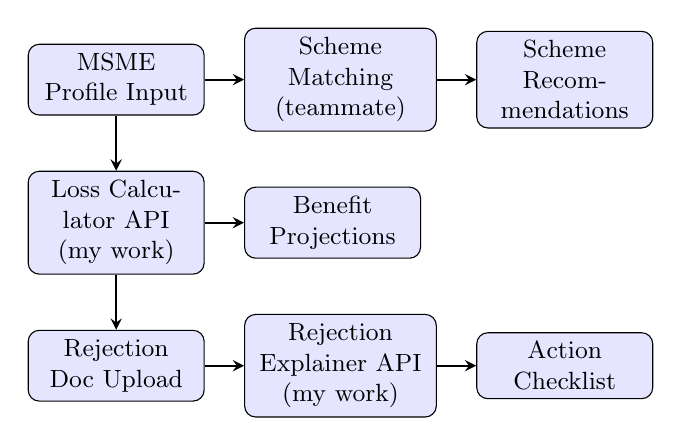
\begin{tikzpicture}[node distance=0.4cm and 0.5cm]
  \node (profile) [block, text width=2cm] {MSME Profile Input};
  \node (match)   [block, right=of profile, text width=2.2cm] {Scheme Matching (teammate)};
  \node (recs)    [block, right=of match, text width=2cm] {Scheme Recommendations};
  \node (calc)    [block, below=0.7cm of profile, text width=2cm] {Loss Calculator API (my work)};
  \node (proj)    [block, right=of calc, text width=2cm] {Benefit Projections};
  \node (upload)  [block, below=0.7cm of calc, text width=2cm] {Rejection Doc Upload};
  \node (explain) [block, right=of upload, text width=2.2cm] {Rejection Explainer API (my work)};
  \node (action)  [block, right=of explain, text width=2cm] {Action Checklist};

  \draw[arrow] (profile) -- (match);
  \draw[arrow] (match)   -- (recs);
  \draw[arrow] (profile.south) -- (calc.north);
  \draw[arrow] (calc)    -- (proj);
  \draw[arrow] (calc.south) -- (upload.north);
  \draw[arrow] (upload)  -- (explain);
  \draw[arrow] (explain) -- (action);
\end{tikzpicture}
\caption{AdhikarSetu -- User Workflow}
\label{fig:adhi_flow}
\end{figure}

\section{Results and Practical Applications}

\par\noindent The platform successfully demonstrated scheme discovery, financial benefit estimation, rejection analysis, and interactive analytics. It serves MSME owners seeking to identify relevant benefits, businesses aiming to understand rejection notices, policymakers analyzing participation trends, and government agencies identifying underserved regions. Future development will integrate PostgreSQL storage, machine learning-based eligibility scoring, and multilingual document processing.

%% ============================================================
%% CHAPTER 5: STOCK INTELLIGENCE DASHBOARD
%% ============================================================
\chapter{Stock Intelligence Dashboard}

\section{Project Overview and Objective}

\par\noindent \textbf{Project Title:} Stock Intelligence Dashboard -- AI-Powered Stock Analysis and Prediction Platform\\
\textbf{Live URL:} \href{https://smart-stock18.vercel.app}{smart-stock18.vercel.app}

\par\noindent \textbf{Problem Statement:} Retail investors rely on multiple disconnected tools for market analysis. Most platforms provide raw prices without intelligent analysis, and none integrate ML-based prediction, conversational AI, multilingual support, and interactive visualization in a single application.

\par\noindent \textbf{Objective:} To build a production-ready stock intelligence platform providing real-time data, ML ensemble price forecasting, AI-assisted research reports, BYOK multi-provider chat, and multilingual support. This was a fully individual project.

\section{System Architecture and Tech Stack}

\begin{table}[!h]
\begin{center}
\small
\begin{tabular}{|l|l|}
\hline
\textbf{Layer} & \textbf{Technology} \\
\hline
Backend Framework & FastAPI (Python 3.11), Uvicorn \\
ML Library & scikit-learn (Linear Regression, Random Forest) \\
Data Source & Yahoo Finance (primary), Finnhub (company metadata) \\
Database & Supabase PostgreSQL \\
Frontend & React 18, TypeScript, Vite, Tailwind CSS \\
State / Data Fetching & Zustand, TanStack Query \\
Charts & Plotly \\
Internationalization & i18next (EN, HI, OD, DE, FR) \\
PDF Export & jsPDF + html2canvas \\
Deployment & Railway (backend), Vercel (frontend), Docker \\
CI/CD & GitLab Pipelines (lint, type-check, test, Docker build) \\
AI Providers & Groq, OpenAI, Anthropic, Gemini, OpenRouter, Ollama \\
\hline
\end{tabular}
\caption{Stock Intelligence Dashboard -- Technology Stack}
\label{tab:stock_stack}
\end{center}
\end{table}

\section{Machine Learning Pipeline}

\par\noindent \textbf{Feature Engineering:} The \texttt{FeatureEngineer} module computes the features listed in Table~\ref{tab:features}. RSI and EMA are additionally available for chart visualization.

\begin{table}[!h]
\begin{center}
\small
\begin{tabular}{|l|l|}
\hline
\textbf{Feature} & \textbf{Description} \\
\hline
Close, Volume & Raw OHLCV inputs \\
MA7, MA21 & 7-day and 21-day moving averages \\
Returns & Percentage daily return \\
Lag1--Lag5 & Previous 1--5 day closing prices \\
Volume Change & Percentage daily volume variation \\
\hline
\end{tabular}
\caption{ML Feature Set}
\label{tab:features}
\end{center}
\end{table}

\par\noindent \textbf{Prediction Target:} Next trading day closing price ($y = \text{Close}_{t+1}$) using an 80:20 chronological train-test split. Models are cached as \texttt{ticker\_range\_model.pkl} via Joblib with LRU caching to manage Railway memory.

\par\noindent \textbf{Ensemble Arbitration:} Linear Regression and Random Forest produce independent forecasts. When both models predict the same trend direction, a weighted average proportional to confidence scores is used. On disagreement, the higher-confidence model's prediction is accepted and the other discarded. When the confidence difference is less than 0.05, the prediction is flagged as \textit{Low Confidence}.

The confidence score is computed as:
\begin{equation}
  \text{Confidence} = \frac{R^2 + 1}{2} \times \left(1 - \text{RMSE penalty}\right)
\end{equation}

\par\noindent Performance metrics displayed to the user include RMSE, MAE, and $R^2$.

\section{BYOK AI Chat and Report Generation}

\par\noindent The platform implements a Bring-Your-Own-Key (BYOK) architecture. Users may enter their own API keys through the UI for any of the six supported providers (Groq, OpenAI, Anthropic, Gemini, OpenRouter, Ollama). Keys are stored exclusively in browser \texttt{localStorage} and are never persisted in Supabase or transmitted to the backend. A default Groq key is available as fallback.

\par\noindent Each AI conversation is injected with company profile data, historical prices, prediction metrics, and recent candle data as structured context before LLM inference. The platform also auto-generates an 11-section equity research report (executive summary through conclusion) exportable as PDF via jsPDF. Conversation histories are ticker-specific and persisted in \texttt{localStorage}.

\section{Methodology Workflow}

\par\noindent Figure~\ref{fig:stock_flow} shows the end-to-end system workflow.

\begin{figure}[ht]
\centering
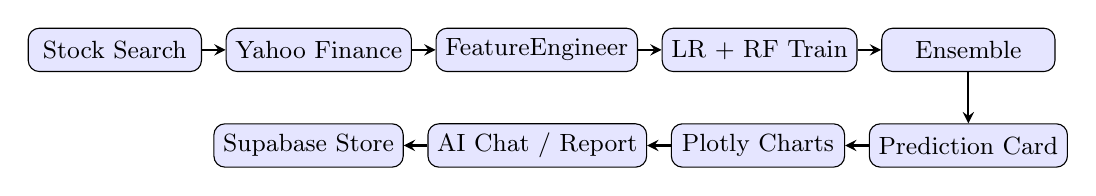
\begin{tikzpicture}[node distance=0.4cm and 0.3cm]
  \node (search) [block] {Stock Search};
  \node (fetch)  [block, right=of search] {Yahoo Finance};
  \node (feat)   [block, right=of fetch] {FeatureEngineer};
  \node (train)  [block, right=of feat] {LR + RF Train};
  \node (ens)    [block, right=of train] {Ensemble};
  \node (pred)   [block, below=0.65cm of ens] {Prediction Card};
  \node (viz)    [block, left=of pred] {Plotly Charts};
  \node (ai)     [block, left=of viz] {AI Chat / Report};
  \node (db)     [block, left=of ai] {Supabase Store};

  \draw[arrow] (search) -- (fetch);
  \draw[arrow] (fetch)  -- (feat);
  \draw[arrow] (feat)   -- (train);
  \draw[arrow] (train)  -- (ens);
  \draw[arrow] (ens)    -- (pred);
  \draw[arrow] (pred)   -- (viz);
  \draw[arrow] (viz)    -- (ai);
  \draw[arrow] (ai)     -- (db);
\end{tikzpicture}
\caption{Stock Intelligence Dashboard -- System Workflow}
\label{fig:stock_flow}
\end{figure}

\section{Database Design}

\par\noindent Supabase PostgreSQL stores watchlists, search history, prediction records (predicted price, actual price, confidence, model name), and saved model metadata. Historical prices, chat history, and API keys are intentionally excluded from server-side storage for privacy and performance reasons.

\section{Results and Practical Applications}

\par\noindent The deployed platform successfully integrates stock data retrieval, ML prediction, AI-assisted analysis, and multilingual access. The ensemble arbitration mechanism provides more stable predictions than either model independently. The BYOK architecture makes the platform LLM-agnostic and cost-transparent. The GitLab CI/CD pipeline enforces code quality through formatting, linting, type-checking, security scanning, and coverage thresholds above 80\%.

\par\noindent Future enhancements include directional accuracy tracking, multi-day prediction horizons, backtesting frameworks, portfolio-level analysis, and an authenticated user system with persistent preferences.

%% ============================================================
%% CHAPTER 6: SEMINARS, WORKSHOPS AND LEARNING
%% ============================================================
\chapter{Technical Learning and Professional Development}

\par\noindent The PS-I period at Swecha Telangana included structured sessions, workshops, and collaborative activities that contributed substantially to technical growth beyond the four projects. This chapter summarizes the key learning outcomes across domains.

\section{Version Control and Collaborative Development}

\par\noindent Intensive practical exposure to Git and GitHub reinforced foundational version control concepts including branching strategies, merging workflows, and pull request-based code review. Working across all four projects with separate GitLab and GitHub repositories instilled discipline in commit hygiene, branch naming conventions, and repository management. GitLab CI/CD pipeline design for the Stock Dashboard deepened understanding of automated testing, build pipelines, and release workflows.

\section{AI and Machine Learning Fundamentals}

\par\noindent Sessions on AI fundamentals covered the architecture of Large Language Models, the Retrieval-Augmented Generation paradigm, embedding spaces, and vector databases. Practical implementation of these concepts in the Document Intelligence Chatbot project consolidated theoretical knowledge into production experience. Exposure to prompt engineering --- including structured prompting, chain-of-thought techniques, and AI-assisted software development using tools such as GitHub Copilot and Lovable --- demonstrated how to productively integrate LLMs into engineering workflows.

\par\noindent Machine learning workshops covering scikit-learn covered regression models, feature engineering pipelines, model evaluation metrics (RMSE, MAE, $R^2$), ensemble methods, and cross-validation. These techniques were directly applied in the Stock Intelligence Dashboard.

\section{Python Ecosystem and Data Engineering}

\par\noindent Workshops on Python, NumPy, and Pandas reinforced data analysis, numerical computing, and structured dataset manipulation. Supabase was explored as a backend-as-a-service platform combining PostgreSQL storage with a REST API layer, providing practical experience in database schema design and integration. Streamlit sessions demonstrated rapid application development for ML-backed interfaces, directly applied in the Document Intelligence Chatbot.

\section{Web Development and Deployment}

\par\noindent The PS-I period deepened understanding of full-stack web development spanning React, Next.js, FastAPI, and deployment infrastructure. Practical exposure to Docker containerization, Vercel and Railway deployment platforms, and CI/CD configuration established a coherent mental model of the software delivery lifecycle. Internet security concepts including HTTPS, REST API design, authentication principles, and secure key management were reinforced through the BYOK architecture of the Stock Dashboard.

\section{Civic Technology and Community Engagement}

\par\noindent The AdhikarSetu hackathon introduced specification-driven development practices, including structured requirement gathering, rapid prototyping, and agile project planning under time constraints. OpenStreetMap sessions introduced open geographic data, community-driven datasets, and mapping concepts applicable to civic technology solutions. Participation in a medical camp organized at Swecha provided experience in community coordination, volunteering, and the practical aspects of social responsibility within a technology organization.

\section{Developer Experience and Professional Practices}

\par\noindent Across all projects, systematic attention was paid to project structure, debugging methodology, code quality tooling (ESLint, Ruff, Pyright), and documentation practices. These activities collectively reinforced the value of maintainable, well-documented codebases and structured engineering workflows.

%% ============================================================
%% CHAPTER 7: CONCLUSIONS
%% ============================================================
\chapter{Conclusions}

\par\noindent Practice School-I at Swecha Telangana provided a comprehensive and intensive engineering experience. The four projects collectively spanned frontend engineering with advanced animations, retrieval-augmented generation with NLP analytics, civic technology with backend API development, and production-grade machine learning with financial analytics.

\par\noindent Each project required end-to-end ownership --- from requirement analysis and system design through implementation, testing, and deployment --- which significantly accelerated professional development beyond what classroom instruction alone provides.

\par\noindent The most technically demanding project, the Stock Intelligence Dashboard, demonstrated the feasibility of building a production-ready, multi-provider AI platform with an ML prediction pipeline, real-time data integration, and cloud-native deployment within a constrained timeline. The AdhikarSetu project reinforced the importance of clear contribution delineation in collaborative environments and the challenges of building civic technology for under-resourced user groups.

\par\noindent The learning outcomes from workshops and seminars --- spanning Git workflows, prompt engineering, ML fundamentals, Python data engineering, and security practices --- form a solid foundation for advanced software engineering in the remaining years of the degree programme.

\bibliography{ref}
\addcontentsline{toc}{chapter}{Bibliography}

\begin{appendices}
\chapter{Project URLs and Repositories}
\begin{itemize}
  \item HighOnCode Portfolio: \href{https://highoncode.vercel.app}{highoncode.vercel.app}
  \item Document Intelligence Chatbot: \href{https://code.swecha.org/soumyajit_07/meowbot}{code.swecha.org/soumyajit\_07/meowbot}
  \item AdhikarSetu: \href{https://adhikarsetu.vercel.app}{adhikarsetu.vercel.app}
  \item Stock Intelligence Dashboard: \href{https://smart-stock18.vercel.app}{smart-stock18.vercel.app}
\end{itemize}
\end{appendices}

\end{document}
